\documentclass[tikz,border=10pt]{standalone}
\usepackage{tikz}
\usetikzlibrary{shapes.geometric,shapes.symbols,arrows,positioning}
\begin{document}

% \begin{figure}[htbp]
% \centering
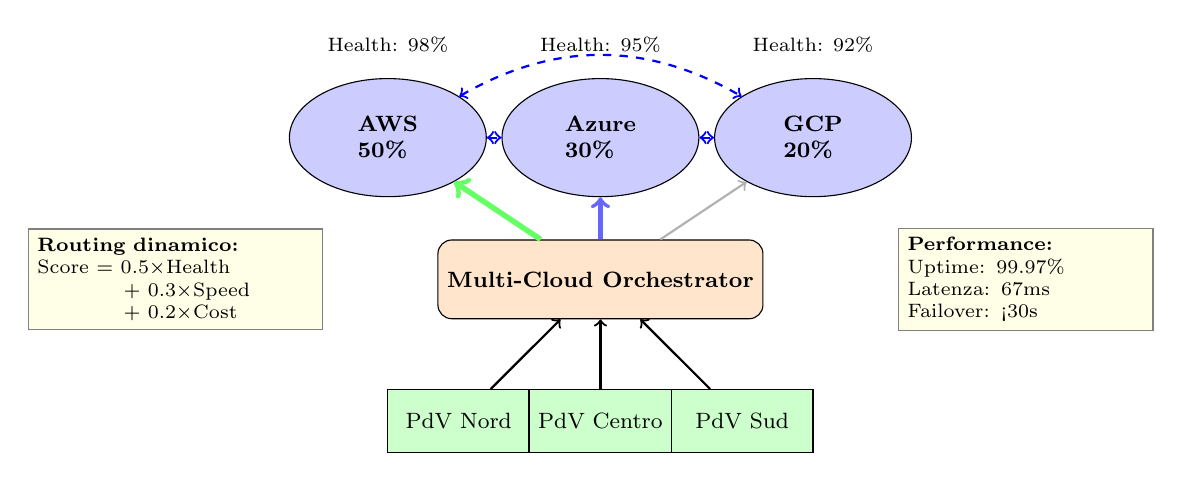
\begin{tikzpicture}[
    scale=0.9,
    cloud/.style={
        ellipse, draw=black, fill=blue!20, 
        minimum width=2.5cm, minimum height=1.5cm,
        font=\footnotesize\bfseries
    },
    orchestrator/.style={
        rectangle, draw=black, fill=orange!20,
        minimum width=4cm, minimum height=1cm,
        rounded corners=5pt, font=\footnotesize\bfseries
    },
    store/.style={
        rectangle, draw=black, fill=green!20,
        minimum width=1.8cm, minimum height=0.8cm,
        font=\footnotesize
    },
    metric/.style={
        rectangle, draw=gray, fill=yellow!10,
        minimum width=2cm, minimum height=0.6cm,
        font=\scriptsize
    },
    arrow/.style={->, thick},
    sync/.style={<->, thick, dashed, blue}
]

% Cloud Providers
\node[cloud, align=left] (aws) at (-3,4) {AWS\\50\%};
\node[cloud, align=left] (azure) at (0,4) {Azure\\30\%};
\node[cloud, align=left] (gcp) at (3,4) {GCP\\20\%};

% Health Score sopra ogni cloud
\node[above=0.2cm of aws, font=\scriptsize] {Health: 98\%};
\node[above=0.2cm of azure, font=\scriptsize] {Health: 95\%};
\node[above=0.2cm of gcp, font=\scriptsize] {Health: 92\%};

% Orchestrator
\node[orchestrator] (orch) at (0,2) {Multi-Cloud Orchestrator};

% Sincronizzazione dati
\draw[sync] (aws) -- (azure);
\draw[sync] (azure) -- (gcp);
\draw[sync] (aws) to[bend left=30] (gcp);

% Connessioni a orchestrator
\draw[arrow, green!60, line width=2pt] (orch) -- (aws);
\draw[arrow, blue!60, line width=1.5pt] (orch) -- (azure);
\draw[arrow, gray!60] (orch) -- (gcp);

% Punti vendita
\node[store] (pv1) at (-2,0) {PdV Nord};
\node[store] (pv2) at (0,0) {PdV Centro};
\node[store] (pv3) at (2,0) {PdV Sud};

% Connessioni dai PdV
\draw[arrow] (pv1) -- (orch);
\draw[arrow] (pv2) -- (orch);
\draw[arrow] (pv3) -- (orch);

% Box metriche (semplificato)
\node[metric, text width=3cm, align=left] at (6,2) {
    \textbf{Performance:}\\
    Uptime: 99.97\%\\
    Latenza: 67ms\\
    Failover: <30s
};

% Box algoritmo (semplificato)
\node[metric, text width=3.5cm, align=left] at (-6,2) {
    \textbf{Routing dinamico:}\\
    Score = 0.5×Health\\
    \hspace{1cm} + 0.3×Speed\\
    \hspace{1cm} + 0.2×Cost
};

\end{tikzpicture}
% \caption{Pattern Multi-Cloud Resilience con bilanciamento dinamico. L'orchestratore distribuisce il traffico tra tre cloud provider basandosi su health score real-time. La sincronizzazione dati garantisce consistenza, mentre il failover automatico assicura continuità in <30 secondi.}
% \label{fig:multicloud_pattern}
% \end{figure}
\end{document}